\section{Bürstenloser Gleichstrommotor BLDC}
Bürstenlose Gleichstrommotoren werden mit Gleichstrom betrieben, oft auch mit einem Akku. Solche Motoren werden jedoch mit Steuerelektronik versehen, um aus der Gleichspannung ein passendes Drehfeld zu erzeugen, anders als bei Gleichstrommaschinen mit Kohleschleifern. In diesem Kapitel wird näher auf diese Art von Gleichstrommaschine eingegangen. 
\cite{wiki:BLDC}

\subsection{Grundlegende Funktionen}
Bei einem bürstenlosen Gleichstrommotor befinden sich im Rotor (beweglicher Teil) Permanentmagneten und im Stator (feststehender Teil) die Spulen. Für gewöhnlich sind die Wicklungen mit drei Phasen versorgt, es gibt aber auch BLDC-Motoren mit einer geringeren Anzahl an Phasen. Bürstenlose Gleichstrommotoren werden als genutete Wicklung ausgeführt, der Wicklungsdraht wird um einen Eisenkern gewickelt, um die magnetischen Feldlinien gezielter und verdichteter austreten zu lassen. 
\cite{wiki:BLDC}

\subsection{Innenläufer}
Die häufigste Aufbauform ist der Innenläufer. Hier wird der Stator des Motors mit Wicklungen bestückt und um den Rotor geführt. Diese werden fast ausschlie{\ss}lich in genuteter Bauform produziert, doch bei sehr kleinen Motoren ist es möglich die Wicklungen flach auf kreisförmige Bleche aufzukleben beziehungsweise einzugie{\ss}en. Bei dieser Form des BLDC-Motors ist kein Eisenkern vorhanden, was dazu führt, dass die Induktivität der Spulen gering ist und der Stromanstieg der Spulen sehr hoch sein kann. Vorteile der Ausführung als Innenläufer sind das geringe Trägheitsmoment und die leichtere Abfuhr der Verlustwärme, mit diesen Aufbauformen sind generell hohe Drehzahlen möglich. Nachteile einer solchen Maschine sind, dass das erzeugte Drehmoment nicht so hoch werden kann, wie bei anderen Bauformen, und die laufenden Kosten beziehungsweise die Wartung sind teurer. 

\cite{nanotec:BLDC}
\cite{lgeeks:BLDC}

\subsection{Au{\ss}enläufer}
Eine weitere oft produzierte Aufbauform ist der Au{\ss}enläufer. Hier werden am Stator des Motors Wicklungen verbaut und dieser wird in einem glockenförmigen Rotor angebracht, der Rotor läuft also au{\ss}en um den Stator. Diese Form wird nur in genuteter Bauform ausgeführt. Die Mehrzahl der Anwendungen mit Au{\ss}enläufern sind solche in denen viele Motoren gebraucht werden, da diese günstiger zu produzieren sind. Ein weiterer Vorteil ist das hohe Drehmoment, das aufgewendet werden kann, zusätzlich sind sie sehr wartungsarm. Nachteile dieser Ausführung sind die schlechte Temperaturableitung, ein hohes Anlaufmoment und das schlechte dynamische Verhalten aufgrund des hohen Trägheitsmoments. 
\cite{nanotec:BLDC}
\cite{lgeeks:BLDC}
\begin{figure}[h]
    \begin{center}
        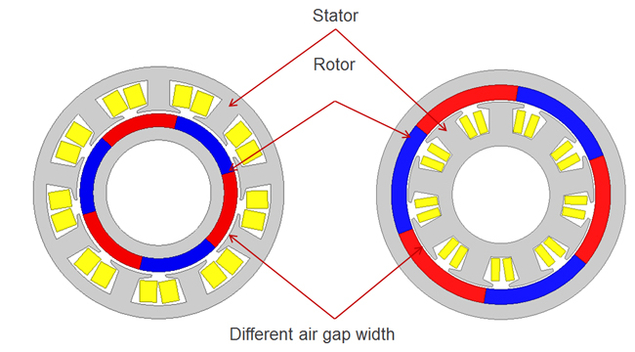
\includegraphics[width=11cm, height= 6cm]{images/Abbildung1.jpg}
        \caption{Innenläufer links – Au{\ss}enläufer rechts 
        \cite{cdyn:BLDC}}
        \label{Innen/Aussenlaeufer}
        \end{center}
\end{figure}

\subsection{Kommutierung}
Die typischste Art, um einen BLDC anzusteuern ist die Kommutierung. Bei dieser Art wird jede Spule abwechselnd ein- und ausgeschaltet, während zwei Spulen aktiv sind, ist eine Spule inaktiv. So kann auch mit Gleichspannung ein Drehfeld erzeugt werden. 
\begin{figure}[h]
    \begin{center}
        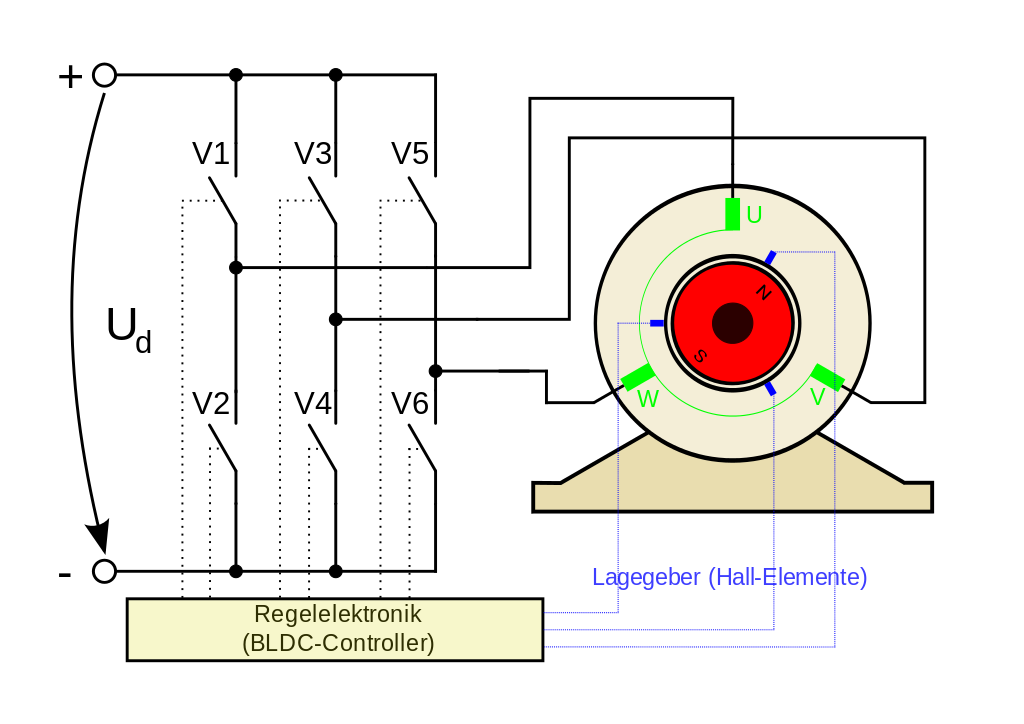
\includegraphics[width=15.35cm, height= 10.85cm]{images/Abbildung 2.png}
        \caption{Dreiphasen Brückenschaltung am BLDC Motor 
        \cite{wiki:BLDC}}
        \label{BrückenschaltungBLDC}
        \end{center}
\end{figure}
Wie in Abbildung 2 werden zum Ein- und Ausschalten drei Halbbrücken verwendet. Als Schalter werden Metal-Oxide Semiconductor Field-Effect Transistor (MOSFET’s) oder Isolated Gate Bipolar Transistors (IGBT’s) verwendet. Durch abwechselndes Durchschalten der Transistoren werden jeweils zwei Wicklungen versorgt und somit wird ein Drehfeld erzeugt. 
\cite{wiki:BLDC}
\cite{sflix:Kommutierung}
\subsubsection{Sensorgesteuerte Kommutierung}
Bei der sensorgesteuerten Kommutierung wird die Rotorposition durch Sensoren erfasst. Sensoren, die verwendet werden können, sind beispielsweise Hall-Sensoren. Diese erkennen die aktuelle Rotorposition durch das Erfassen des magnetischen Flusses. Au{\ss}erdem können optische Sensoren verwendet werden, die am Stator angebracht sind und somit die Position des Rotors erkennen.  Durch die Informationen, die durch das Auslesen dieser Sensoren bereitstehen, kann die Steuerelektronik richtig gesteuert werden, zusätzlich ist es möglich mit solchen Sensoren die Drehzahl zu ermitteln. 
\cite{wiki:BLDC}
\cite{sflix:Kommutierung}
\clearpage
\subsubsection{Sensorlose Kommutierung}
Wenn keine Sensoren verwendet werden, dann handelt es sich um eine sensorlose Kommutierung. Die Spulen werden durch das Erfassen von elektrischen Grö{\ss}en ein- und ausgeschaltet. Diese elektrischen Grö{\ss}en sind beispielsweise Motorstrom- oder Spannung. Aufgrund dieser Grö{\ss}en wird auf die aktuelle Geschwindigkeit des Motors geschlossen und der Kommutierungsblock richtig geschalten. Ein Problem der sensorlosen Kommutierung ist, dass ein Minimum an Drehzahl erreicht werden muss, um eine Gegenspannung im Rotor messen zu können. Diese Art der Kommutierung hat zur Folge, dass beim Anlauf der Maschine blind geschaltet werden muss. 
\cite{wiki:BLDC}
\cite{SPSM:SLKomm}
\subsection{Einsatzbereiche von bürstenlosen Gleichstrommotoren}
BLDC-Motoren haben unzählige Einsatzbereiche einige Beispiele sind: \cite{wiki:BLDC}
\begin{itemize}
    \item Festplatten für PCs und andere Laufwerke, wie DVD oder Blu-Ray \cite{ASPINA:BLDC}
    \begin{itemize}
        \item Diese Motoren werden hier aufgrund ihrer hohen Präzision verwendet. \cite{ASPINA:BLDC}
\end{itemize}
\end{itemize}
\begin{itemize}
    \item E-Mobility \cite{wiki:BLDC}
    \begin{itemize}
        \item Autohersteller nutzen diese Motoren, da sie ohne gro{\ss}en Aufwand mit einem Akku betrieben werden können. 
         Und oft sehr leicht sind. \cite{wiki:BLDC}
        \item Aus diesem Grund werden solche Motoren in der Emily verwendet. 
\end{itemize}
\end{itemize}
\begin{itemize}
    \item Werkzeuge mit Akku \cite{wiki:BLDC}
    \begin{itemize}
        \item Werkzeughersteller tendieren zu BLDC-Motoren, da diese weniger Wartungen als Motoren mit Bürsten benötigen. \cite{wiki:BLDC}
\end{itemize}
\end{itemize}
